\documentclass[sigconf]{acmart}
\usepackage{lipsum}

% Local Commands
\newcommand{\ucscaffil}{\affiliation{\institution{University of California, Santa Cruz}\streetaddress{1156 High St - 95064}\city{Santa Cruz, CA}\country{U.S.A.}}}

% Document Configuration
\setcopyright{acmcopyright}
\copyrightyear{2019}
\acmYear{N/A}

\acmConference[Santa Cruz '19]{UC Santa Cruz '19: CMPM 163, Spring Quarter 2019}{June 01--13, 2019}{Santa Cruz, CA}
\acmBooktitle{UC Santa Cruz '19: CMPM 163 Final Project, June 01--13, 2019, Santa Cruz, CA}
\acmPrice{0.00}
\acmISBN{?????????}

\begin{document}

% TITLE CONFIGURATION
\title{VFX Demonstration: Close Encounter of the Second Kind}

\author{Anthony Medina}
\authornote{ROLE}
\email{amedin12@ucsc.edu}
\ucscaffil

\author{Jan Yu}
\authornote{ROLE}
\email{jyu92@ucsc.edu}
\ucscaffil

\author{Malcolm Riley}
\authornote{ROLE}
\email{masriley@ucsc.edu}
\ucscaffil

\renewcommand{\shortauthors}{Medina, Yu, and Riley}

\begin{abstract}
	\lipsum[1]
\end{abstract}

\begin{CCSXML}
<ccs2012>
	<concept>
		<concept_id>10010147.10010341</concept_id>
		<concept_desc>Computing methodologies~Modeling and simulation</concept_desc>	
		<concept_significance>500</concept_significance>
	</concept>
	<concept>
		<concept_id>10003120.10003145</concept_id>
		<concept_desc>Human-centered computing~Visualization</concept_desc>
		<concept_significance>500</concept_significance>
	</concept>
		<concept>
		<concept_id>10003120.10003121</concept_id>
		<concept_desc>Human-centered computing~Human computer interaction (HCI)</concept_desc>
		<concept_significance>100</concept_significance>
	</concept>
</ccs2012>
\end{CCSXML}

\ccsdesc[500]{Computing methodologies~Modeling and simulation}
\ccsdesc[500]{Human-centered computing~Visualization}
\ccsdesc[100]{Human-centered computing~Human computer interaction (HCI)}

\keywords{keywords,keywords,keywords}

%\begin{teaserfigure}
%	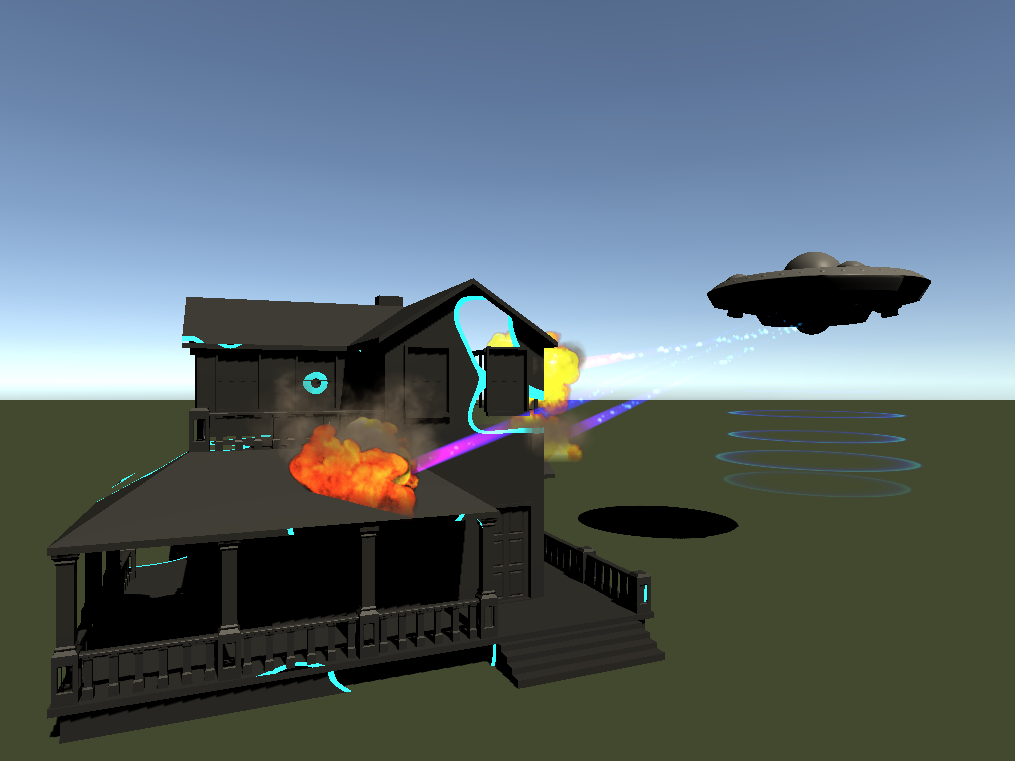
\includegraphics[width=\textwidth]{images\teaser}
%	\caption{CAPTION}
%	\Description{DESCRIPTION}
%	\label{fig:teaser}
%\end{teaserfigure}

% TITLE
\maketitle

% INTRODUCTION
\section{Introduction}
\lipsum[1]

\section{VFX Explanation 1}

\subsection{Methodology}
\lipsum[2]
\subsection{Implementation}
\lipsum[5-7]
\subsection{Result}
\lipsum[9]

\section{VFX Explanation 2}

\subsection{Methodology}
\lipsum[2]
\subsection{Implementation}
\lipsum[5-7]
\subsection{Result}
\lipsum[9]

\section{VFX Explanation 3}

\subsection{Methodology}
\lipsum[2]
\subsection{Implementation}
\lipsum[5-7]
\subsection{Result}
\lipsum[9]

%\begin{figure}[h]
%	\centering
%	\includegraphics[width=\linewidth]{images/figure}
%	\caption{1907 Franklin Model D roadster. Photograph by Harris \& Ewing, Inc. [Public domain], via Wikimedia Commons. (\url{https://goo.gl/VLCRBB}).}
%	\Description{The 1907 Franklin Model D roadster.}
%\end{figure}

\begin{acks}
	\lipsum[3]
\end{acks}

\bibliographystyle{ACM-Reference-Format}
\bibliography{citations}

\appendix
\lipsum

\end{document}